% fs-06-PoissonNormal.tex

\documentclass[xcolor=dvipsnames]{beamer}
\usepackage{teachbeamer}

\title{The Poisson and the Normal Distribution}
\subtitle{{\CourseNumber}, BCIT}

\author{\CourseName}

\date{February 8, 2018}

% \begin{figure}[h]
% 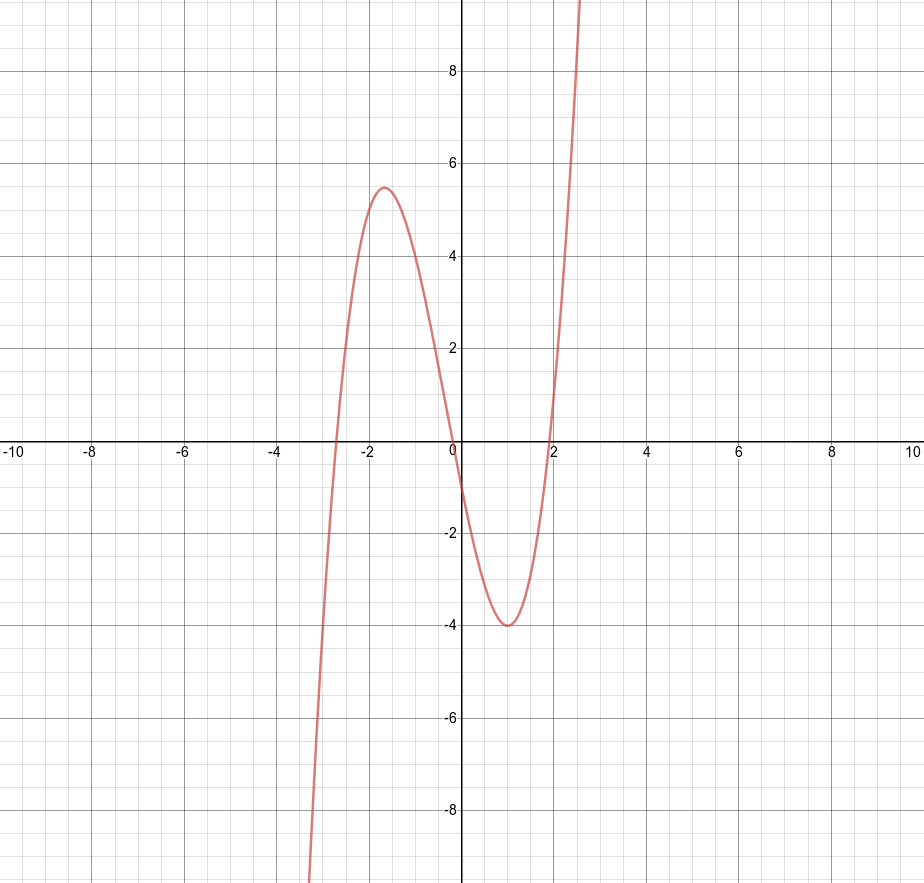
\includegraphics[scale=.3]{./diagrams/extrema1.png}
% \end{figure}

% Command             10pt    11pt    12pt
% \tiny               5       6       6
% \scriptsize         7       8       8
% \footnotesize       8       9       10
% \small              9       10      10.95
% \normalsize         10      10.95   12

\begin{document}

\begin{frame}
  \titlepage
\end{frame}

\begin{frame}
  \frametitle{Poisson Distribution}
The \alert{Poisson Distribution} is another discrete probability
distribution. It applies to occurrences of some event over a specified
interval, such as time or distance. The probability of the event
occurring $x$ times over an interval is given by
\begin{equation}
  \label{eq:zaengeit}
  P(X=x)=\frac{\lambda^{x}\cdot{}e^{-\lambda}}{x!}
\end{equation}
where $e$ is Euler's number ($\approx{}2.71828$) and $\lambda$ is the mean
number of occurrences over the interval.
\end{frame}

\begin{frame}
  \frametitle{Poisson Distribution Example}
\beispiel{Earthquakes} The mean number of annual major earthquakes
in the world is 0.93. Calculate the probability of $x$ earthquakes
happening in one year.

\medskip

\begin{tabular}{|r|r|r|}\hline
  Number of Earthquakes & Poisson Distribution & Actual Figure \\ \hline 
  0                     & 0.3946               & 47 out of 100 \\ \hline
  1                     & 0.3669               & 31 out of 100 \\ \hline
  2                     & 0.1706               & 13 out of 100 \\ \hline
  3                     & 0.0529               & 5 out of 100  \\ \hline
  4                     & 0.0123               & 2 out of 100  \\ \hline
  5                     & 0.0029               & 0 out of 100  \\ \hline
  6                     & 0.0004               & 1 out of 100  \\ \hline
  7                     & 0+                   & 1 out of 100  \\ \hline
\end{tabular}
\end{frame}

% \begin{frame}
%   \frametitle{Poisson Distribution in R}
% In R Statistics, you use the following command to find the poisson distribution. 
% \begin{alltt}
%   dpois(2,lambda=0.93)
% \end{alltt}
% for the probability of $x=2$ with $\lambda=0.93$.
% \begin{alltt}
%   ppois(16,lambda=12)
% \end{alltt}
% for the probability of $x$ being \alert{16 or less} with $\lambda=12$.
% \end{frame}

\begin{frame}
  \frametitle{Summary}
The binomial and Poisson distributions are discrete probability
distributions. The formulas are as follows.
\begin{equation}
  \label{eq:hiechoib}
  \mbox{\textbf{[binomial] }}P(X=x)=\binom{n}{x}\cdot{}p^{x}\cdot(1-p)^{n-x}\mbox{ for }(x,n,p)\notag
\end{equation}
\begin{equation}
  \label{eq:iechahve}
  \mbox{\textbf{[Poisson] }}P(X=x)=\frac{\lambda^{x}\cdot{}e^{-\lambda}}{x!}\mbox{ for }(x,\lambda)\notag
\end{equation}
Use the following functions in R Statistics.
\begin{itemize}
\item $P(X=x)=$\texttt{dbinom(x,n,p)} for binomial, not cumulative.
\item $P(X\leq{}x)=$\texttt{pbinom(x,n,p)} for binomial, cumulative.
\item $P(X=x)=$\texttt{dpois(x,$\lambda$)} for Poisson, not cumulative.
\item $P(X\leq{}x)=$\texttt{ppois(x,$\lambda$)} for Poisson, cumulative.
\end{itemize}
\end{frame}

\begin{frame}
  \frametitle{Exercise I}
  {\ubung} A river causes 15 floods in 100 years in the long run. The
  floods occur independently of each other. What is the probability
  for 3 or more floods to occur in the next 10 years?
\end{frame}

\begin{frame}
  \frametitle{Exercise II}
  {\ubung} Mars Inc. tells us that 20\% of M\&Ms are orange. A bag
  contains 42 M\&Ms. What is the probability of a bag containing
  between 7 and 9 orange M\&Ms?
\end{frame}

\begin{frame}
  \frametitle{Exercise III}
  {\ubung} Over the last 100 million years, 600 climate-changing
  meteors have hit the Earth. What is the probability of one or more
  climate-changing meteors hitting the Earth in the next 100 years?
\end{frame}

\begin{frame}
  \frametitle{Exercise IV}
  {\ubung} The average number of goals in a World Cup soccer match is
  approximately 2.5. What is the probability that a match ends
  scoreless? What is the probability that strictly more than 3 goals
  are scored in a match?
\end{frame}

\begin{frame}
  \frametitle{Exercise V}
  {\ubung} Twenty people each roll a die. What is the probability that
  five of them roll either a one or a two?
\end{frame}

\begin{frame}
  \frametitle{Exercise VI} {\ubung} You get 15 phone calls every day.
  They happen independently of the time of day. What is the
  probability of getting a phone call in the next 25 minutes?
\end{frame}

\begin{frame}
  \frametitle{Approximating Binomial Probabilities I}
Here is the formula for a \alert{binomial} setup with $n$ trials (for example,
$n=2$ coin tosses), probability of success $p$ (for example, $p=0.5$ for the
probability of heads), and $x$ number of successes,
\begin{equation}
  \label{eq:iedohdah}
  P(X=x)=\frac{n!}{(n-x)!x!}p^{x}(1-p)^{n-x}
\end{equation}
where $0!=1$ and $(n+1)!=n!(n+1)$, for example
$4!=1\cdot{}2\cdot{}3\cdot{}4$ (say ``four factorial''). $X$ is a
\alert{random variable}, the number that the random process spits out.
\end{frame}

\begin{frame}
  \frametitle{Approximating Binomial Probabilities II}
Here are the binomial probabilities for $n=6$. One way to
conceptualize these numbers is by looking at Pascal's Triangle (next
slide). 
  \begin{figure}[h]
    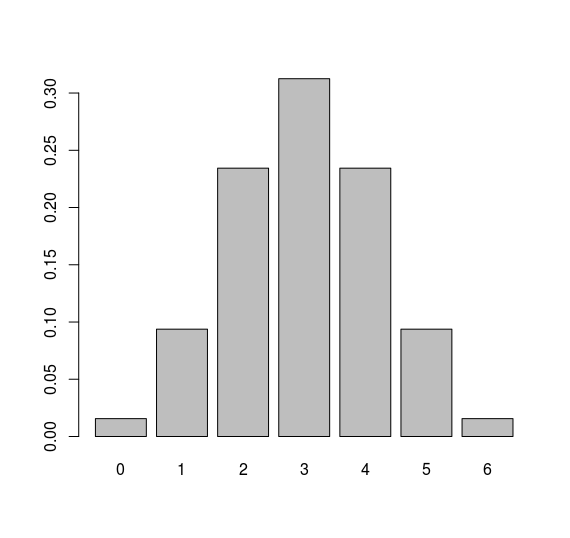
\includegraphics[scale=.5]{./diagrams/binomial1.png}
  \end{figure}
\end{frame}

\begin{frame}
  \frametitle{Pascal's Triangle}
\begin{tikzpicture}
\foreach \n in {0,...,7} {
  \foreach \k in {0,...,\n} {
    \node at (\k-\n/2,-\n) {$\binomialCoefficient{\n}{\k}$};
  }
}
\end{tikzpicture}
\end{frame}

\begin{frame}
  \frametitle{Pascal's Triangle}
\begin{tikzpicture}
\foreach \n in {0,...,7} {
  \foreach \k in {0,...,\n} {
    \node at (\k-\n/2,-\n) {$\binom{\n}{\k}$};
  }
}
\end{tikzpicture}
\end{frame}

\begin{frame}
  \frametitle{Approximating Binomial Probabilities III}
Binomial probabilities are difficult to calculate for high numbers. We
approximate the binomial distribution with the \alert{normal distribution}.
Compare the binomial distribution for $n=10$ with the normal
distribution.
  \begin{figure}[h]
    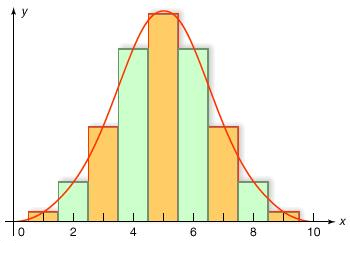
\includegraphics[scale=.5]{./diagrams/binnorm1_ed.jpg}
  \end{figure}
\end{frame}

\begin{frame}
  \frametitle{Normal Distribution}
  The normal probabilities distribution is a \alert{continuous}
  probabilities distribution. There is not just one normal
  distribution. There are infinitely many, characterized by their
  \alert{mean $\mu$} and their \alert{standard deviation $\sigma$}.
  The formula for the normal distribution is
  \begin{equation}
    \label{eq:aitoolah}
    f(x)=\frac{1}{\sigma\sqrt{2\pi}}e^{-(x-\mu)^{2}/(2\sigma^{2})}
  \end{equation}
  \begin{figure}[h]
    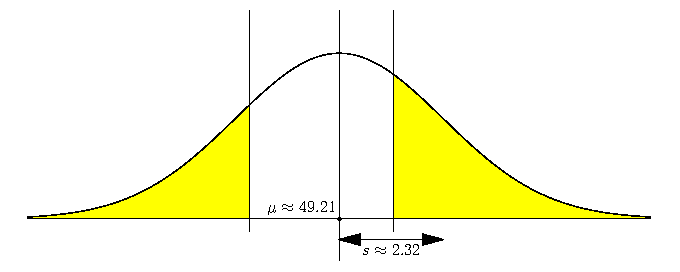
\includegraphics[scale=.4]{./diagrams/qfour.png}
  \end{figure}
\end{frame}

\begin{frame}
  \frametitle{Z Scores}
  To calculate the area under the curve, we carry around a piece of
  paper with all the values for the \alert{standard normal
    distribution} and then convert to the normal distribution with the
  relevant $\mu$ and $\sigma$. The value for the normal distribution
  is called the \alert{$x$-score} and its associate value for the
  standard normal distribution is called the \alert{$z$-score}. Travel
  back and forth using the following formula,
  \begin{equation}
    \label{eq:uotoogoo}
    z=\frac{x-\mu}{\sigma}
  \end{equation}
\end{frame}

\begin{frame}
  \frametitle{Normal Distribution Example Question}
  \beispiel{Men's Heights} The height of adult men is normally
  distributed with mean $\mu=69.5$ inches and standard deviation
  $\sigma=2.4$ inches. What percentage of the adult male population is
  taller than six feet (72 inches)? 
\end{frame}

\begin{frame}
  \frametitle{Normal Distribution Example Answer}
  Find the $z$-score, using the formula
  \begin{equation}
    \label{eq:igutheib}
    z=\frac{x-\mu}{\sigma}=\frac{72-69.5}{2.4}\approx{}1.04
  \end{equation}
  Use your $z$-score table to find the corresponding
  \alert{$p$-value}, which is the area to the left of the $z$-score
  for the standard normal distribution. In this case the $p$-value is
  $0.8508$. This represents the percentage of the male population that
  is \emph{shorter} than 72 inches. The answer to our question is
  therefore, 14.92\% of men are taller than six feet.
\end{frame}

\begin{frame}
  \frametitle{Normal Distribution Exercises I}
{\ubung} Find the area under the curve for the following sets of
$z$-scores. 
\begin{equation}
  \label{eq:deapheph}
\{z|z\leq{}-1.72\}  
\end{equation}
\begin{equation}
  \label{eq:taedaiga}
\{z|1.96<{}z\}  
\end{equation}
\begin{equation}
  \label{eq:ahraefis}
\{z|-1.55\leq{}z\leq{}-0.81\}
\end{equation}
\end{frame}

\begin{frame}
  \frametitle{Normal Distribution Exercises II}
{\ubung} Find the area under the curve for the
following sets of $x$-scores. 
\begin{equation}
  \label{eq:aequaixe}
\{x|x\leq{}83\},\mu=100,\sigma=15
\end{equation}
\begin{equation}
  \label{eq:oocohdau}
\{x|0.44<x\},\mu=0.5,\sigma=0.2  
\end{equation}
\begin{equation}
  \label{eq:aethohph}
\{x|800\leq{}x\leq{}1200\},\mu=911,\sigma=121
\end{equation}
\end{frame}

\begin{frame}
  \frametitle{Normal Distribution Exercises III}
{\ubung} The time it takes a student to solve a particular math problem is
normally distributed with $\mu=3$ minutes and $27$ seconds and a
standard deviation of $\sigma=59$ seconds. How many students finish
the math problem between 3 and 4 minutes?
\end{frame}

\begin{frame}
  \frametitle{Normal Distribution Exercises IV}
  {\ubung} Scores on a certain intelligence test for children between
  ages 13 and 15 years are approximately normally distributed with
  $\mu=106$ and $\sigma=15$.
  \begin{enumerate}
  \item What proportion of children aged 13 to 15 years old have
    scores on this test above 88?
  \item Enter the score which marks the lowest 30 percent of the
    distribution.
  \item Enter the score which marks the highest 15 percent of the
    distribution.
  \end{enumerate}
When you want to find an $x$-score given a $p$-value, you need to use
your table in reverse and then find the $x$-score given the $z$-score
from the table by using the formula
\begin{equation}
  \label{eq:aedecaba}
  x=z\cdot\sigma+\mu
\end{equation}
\end{frame}

\begin{frame}
  \frametitle{Approximating Binomial Probabilities Example I}
  For large numbers, even high-powered computers cannot calculate the
  binomial probabilities. We use the normal distribution to
  approximate the binomial distribution. 

\bigskip

  \beispiel{Die Rolls} If you roll a die 600 times, what is the
  probability of rolling a six fewer than 80 times? 

\bigskip

  It would take very long to calculate this probability using the
  binomial distribution formula! We use the normal distribution with
  $\mu=np$ and $\sigma=\sqrt{np(1-p)}$ instead. 

\bigskip

  Conventionally, it is only acceptable to approximate the binomial
  distribution by the normal distribution if $np\geq{}5$ and
  $nq\geq{}5$. Otherwise, the binomial and the normal distribution are
  too far apart to provide a useful approximation.
\end{frame}

\begin{frame}
  \frametitle{Approximating Binomial Probabilities Example II}
  We need to make a \alert{continuity correction} and ask ourselves,
  what is the probability for the $x$-score to be 79.5 or less for
  this normal distribution?
  \begin{equation}
    \label{eq:oolojuth}
    z=\frac{x-\mu}{\sigma}=\frac{79.5-100}{9.1287}\approx{}-2.25
  \end{equation}
  The corresponding $p$-value is 0.0122. There is only a 1.22\%
  probability that you will roll fewer than 80 sixes in 600 rolls.
\end{frame}

\begin{frame}
  \frametitle{Continuity Correction}
  % Continuity correction means that when we approximate a whole number
  % $m$ using the continuous normal distribution, we use the interval
  % $[m-0.5,m+0.5]$ to represent this whole number. ``Fewer than 80,''
  % for example, is translated for the approximation as ``less than
  % 79.5.'' ``Fewer than or equal to 80'' is translated as ``less than
  % 80.5.''
  \begin{figure}[h]
    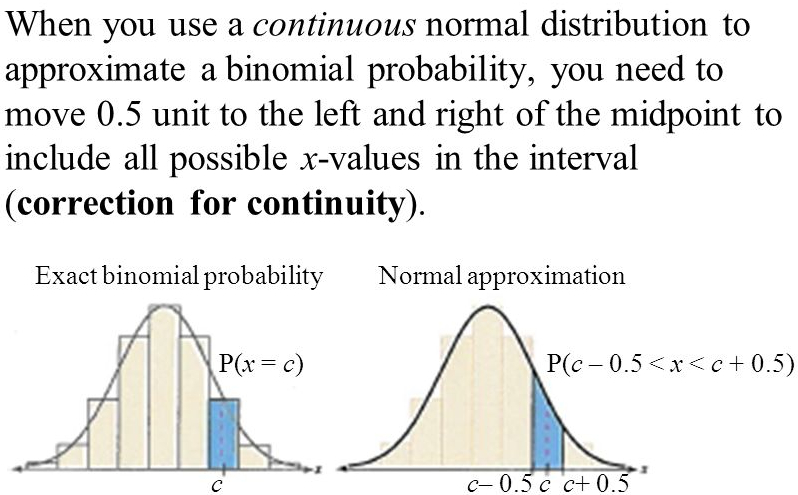
\includegraphics[scale=.5]{./diagrams/contcorr_ed1.jpg}
  \end{figure}
\end{frame}

\begin{frame}
  \frametitle{Binomial Approximation Exercise}
{\ubung} 29\% of a country's population is blue-eyed. What is the
probability that a random sample of 1,000 persons contains between 200
and 300 blue-eyed persons? Approximate the binomial distribution by
the normal distribution. Calculate $\mu=np$ and
$\sigma=\sqrt{np(1-p)}$ for this normal distribution after checking
the conditions $np\geq{}5,n(1-p)\geq{}5$. Then calculate the
$z$-scores for the $x$-scores $x=199.5$ and $x=300.5$. Lastly,
determine the area under the curve between these $z$-scores. Provide a
complete sentence to answer the question.
\end{frame}

\begin{frame}
  \frametitle{Word Problems I}
  The national mortality rate for a particular type of heart surgery
  is 12\%, so you would expect six deaths per 50 operations. You are a
  health administrator, and one of your doctors has had eleven deaths
  in 72 operations. Should you fire her? What is the probability that
  an average surgeon (whose mortality rate is the national average)
  will have twelve or more deaths in 72 operations?

  \bigskip

  You desperately need a person with blood type AB (incidence in
  Canada: 3\%). If there are 49 people in the room, what is the
  probability that at least one of them is AB?
\end{frame}

\begin{frame}
  \frametitle{Word Problems II}
  \begin{figure}[h]
    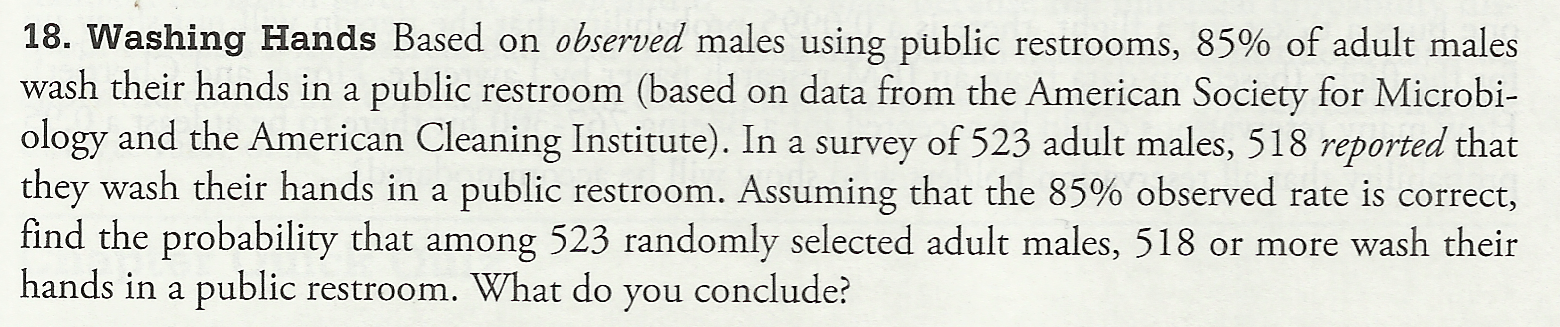
\includegraphics[scale=.7]{./diagrams/triola1.png}
  \end{figure}
  \begin{figure}[h]
    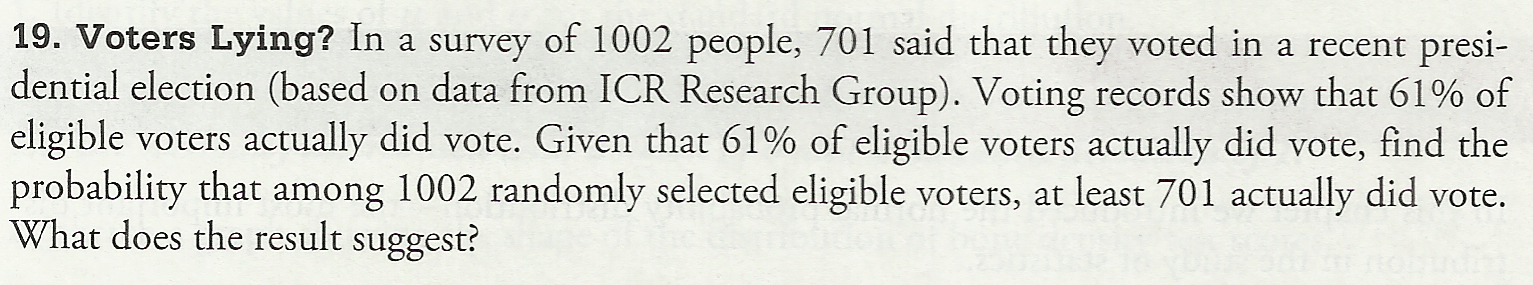
\includegraphics[scale=.7]{./diagrams/triola2.png}
  \end{figure}
  \begin{figure}[h]
    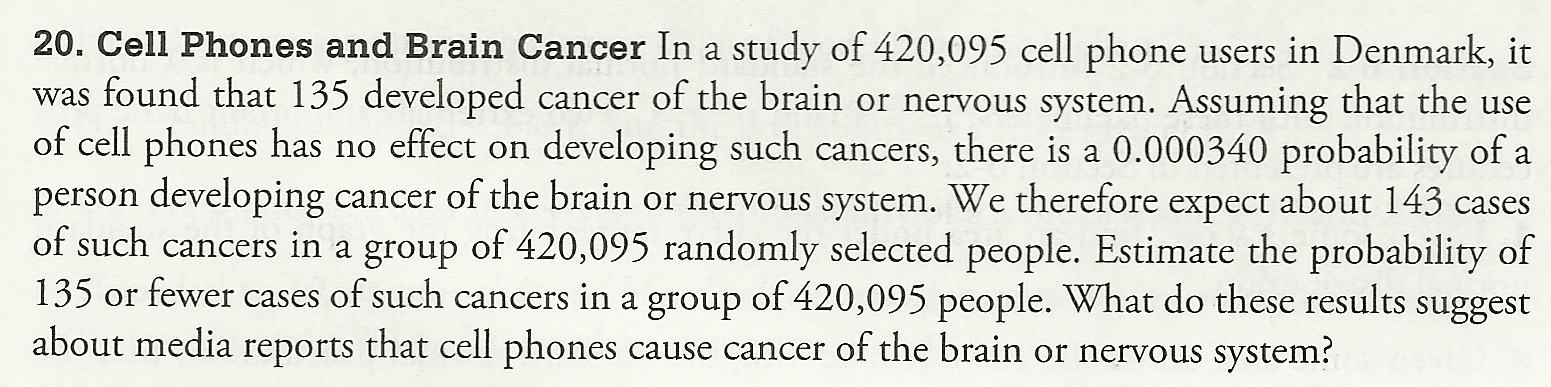
\includegraphics[scale=.7]{./diagrams/triola3.png}
  \end{figure}
\end{frame}

\begin{frame}
  \frametitle{Word Problems III}
  \begin{figure}[h]
    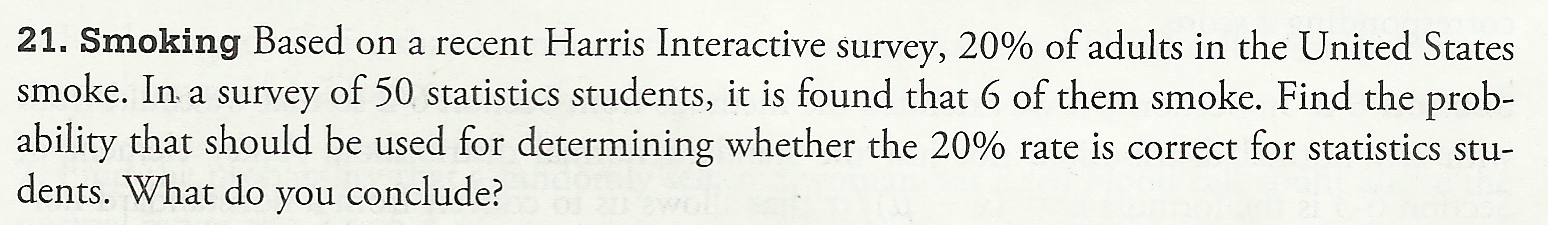
\includegraphics[scale=.7]{./diagrams/triola4.png}
  \end{figure}
  \begin{figure}[h]
    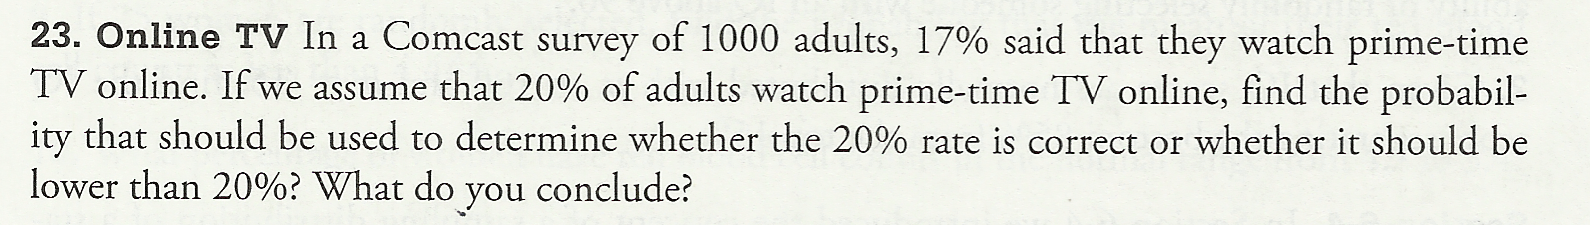
\includegraphics[scale=.7]{./diagrams/triola5.png}
  \end{figure}
  \begin{figure}[h]
    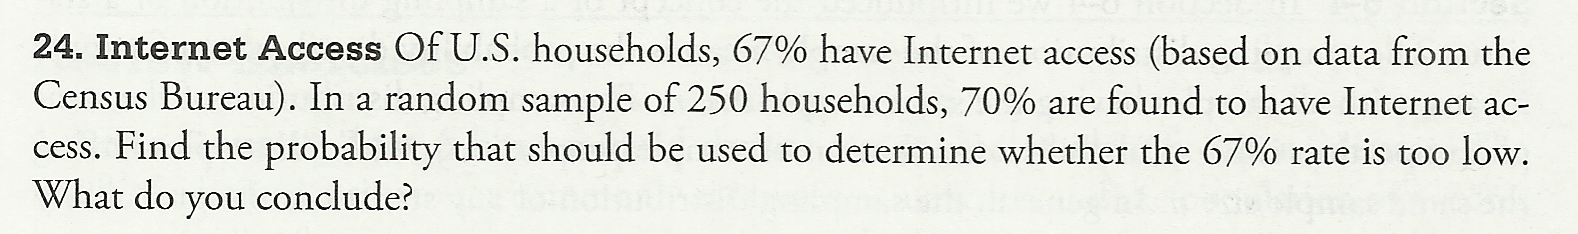
\includegraphics[scale=.7]{./diagrams/triola6.png}
  \end{figure}
\end{frame}

\begin{frame}
  \frametitle{Using Poisson to Approximate Binomial}
% http://courses.wcupa.edu/rbove/Berenson/10th%20ed%20CD-ROM%20topics/section5_6.pdf
  Situations in which $n$ is large and $p$ is very small:
  \begin{enumerate}
  \item I cannot use the binomial formula because my calculator cannot
    handle $n!$.
  \item I cannot use the normal distribution to approximate the
    binomial distribution because $n\cdot{}p<5$.
  \end{enumerate}
  The Poisson distribution can be used to approximate the binomial
  distribution. The larger the $n$ and the smaller the $p$, the better
  the approximation. We use the Poisson distribution for which
  $\lambda=np$.
\end{frame}

\begin{frame}
  \frametitle{Using Poisson to Approximate Binomial}
    \begin{figure}[h]
    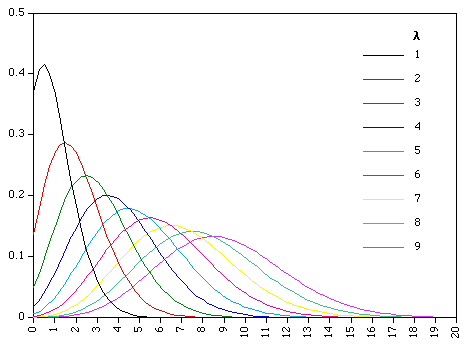
\includegraphics[scale=.62]{./diagrams/poisdist.png}
  \end{figure}
\end{frame}

\begin{frame}
  \frametitle{Using Poisson to Approximate Binomial}
  \beispiel{Manufacturing Tires} Suppose 8\% of the tires manufactured
  at a particular plant are defective. Estimate the probability of obtaining
  exactly one defective tire from a sample of twenty.
  \begin{equation}
    \label{eq:eikaiche}
    P(X=1)^{\mbox{\tiny binomial}}={20\choose{}1}0.08^{1}\cdot0.92^{19}=0.3281623
  \end{equation}
  is approximately
  \begin{equation}
    \label{eq:aihuroot}
    P(X=1)^{\mbox{\tiny poisson}}\frac{e^{-1.6}(1.6)^{1}}{1!}=0.3230344
  \end{equation}
\end{frame}

\begin{frame}
  \frametitle{Using Poisson to Approximate Binomial Exercises}
  {\ubung} Based upon past experience, 1\% of the telephone bills
  mailed to households are incorrect. If a sample of twenty bills is
  selected, find the probability that at least one bill will be
  incorrect. Do this using two probability distributions (the binomial
  and the Poisson) and compare your results.
\end{frame}

\begin{frame}
  \frametitle{Using Poisson to Approximate Binomial Exercises}
  {\ubung} A computer manufacturing company conducts acceptance
  sampling for incoming computer chips. After receiving a huge
  shipment of computer chips, the company randomly selects 800 chips.
  If three or fewer nonconforming chips are found, the entire lot is
  accepted without inspecting the remaining chips in the lot. If four
  or more chips are nonconforming, every chip in the entire lot is
  carefully inspected at the supplier's expense. Assume that the true
  proportion of nonconforming computer chips being supplied is 0.001.
  What is the probability the lot will be accepted?
\end{frame}

\begin{frame}
  \frametitle{Using Poisson to Approximate Binomial Exercises}
  {\ubung} Last month your company sold ten thousand new watches. Past
experience indicates that the probability that a new watch
will  need  repair  during  its  warranty  period  is  0.002.

Compute the probability that:
\begin{enumerate}
\item zero watches will need warranty work
\item no more than 5 watches will need warranty work
\item no more than 10 watches will need warranty work
\item no more than 20 watches will need warranty work
\end{enumerate}
\end{frame}

\begin{frame}
  \frametitle{End of Lesson}
Next Lesson: Sampling Distributions
\end{frame}

\end{document}
